\documentclass[compress]{beamer}
\usepackage{ifthen}

\title{Alignment Monitoring and 1D-Hit Problems}
\author{Jim Pivarski, Dmitry Yakorev, Alexei Safonov}
\institute{Texas A\&M University}
\date{27 April, 2007}

\setbeamertemplate{navigation symbols}{}
\setbeamertemplate{headline}{\includegraphics[height=1 cm]{../cmslogo} \hspace{0.1 cm} \includegraphics[height=1 cm]{../tamulogo} \hfill
\begin{minipage}{9 cm}
\vspace{-0.75 cm} \small
\begin{center}
\ifthenelse{\equal{\insertpagenumber}{1}}{}{\insertsection}
\end{center}
\end{minipage} \hfill
\begin{minipage}{1 cm}
\vspace{-0.75 cm} \small
\begin{center}
\ifthenelse{\equal{\insertpagenumber}{1}}{}{\insertpagenumber/\pageref{numpages}}
\end{center}
\end{minipage}}

\xdefinecolor{verylightgray}{rgb}{0.95,0.95,0.95}
\beamertemplateshadingbackground{verylightgray}{white}

\begin{document}
\frame{\titlepage}

\begin{frame}
\frametitle{Overview of topics}
\begin{description}\setlength{\itemsep}{0.5 cm}
\item[AlignmentProducer Monitoring:] 
\begin{itemize}
\item Alignment/CommonAlignmentMonitor in CVS
\item Structure and features
\end{itemize}

\item[Database Geometry Monitoring:] 
\begin{itemize}
\item Beginnings of an offline tool
\end{itemize}

\item[AlignableDetUnits in the muon system:] 
\begin{itemize}
\item DTs need Gero's fix
\end{itemize}

\item[1D Treatment of DT Hits:] 
\begin{itemize}
\item The ``other'' 1D hits problem
\end{itemize}
\end{description}
\end{frame}

\section*{AlignmentProducer Monitoring --- Jim Pivarski}

\begin{frame}
\frametitle{Alignment/CommonAlignmentMonitor}
\begin{columns}
\column{0.5\linewidth}

Adds histograms, profile plots, and trees to AlignmentProducer
through modular plugins, much like algorithm plugins

\column{0.45\linewidth}
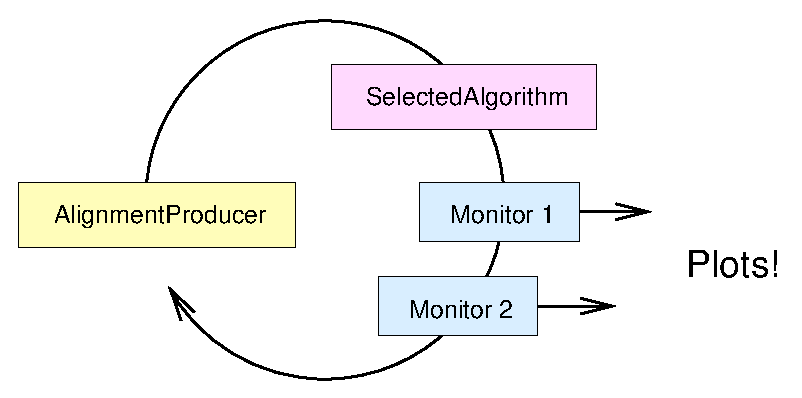
\includegraphics[width=\linewidth]{organization}
\end{columns}

\vfill
Lowers ``potential barrier'' to adding plots
\begin{itemize}
\item AlignmentMonitorBase manages the root file, iteration, and
merging histograms from a distributed job
\item Modularity allows separation of projects by group--- e.g.~CSC~internal alignment doesn't affect tracker studies
\end{itemize}
Expected use:
\begin{itemize}
\item One module for each group, frequently modified in CVS
\item One official module: AlignmentMonitorCSA07
\item We'll rarely use the multiple-modules-in-one-job feature
\end{itemize}
\end{frame}

\begin{frame}
\frametitle{Interface}

{\tt \small
replace AlignmentProducer.monitorConfig = \{ \\
\mbox{\hspace{0.5 cm}}untracked vstring monitors = \{"AlignmentMonitorHIP"\} \\
\mbox{\hspace{0.5 cm}}untracked PSet AlignmentMonitorHIP = \{ \\
\mbox{\hspace{0.5 cm}}\mbox{\hspace{0.5 cm}}string outpath = "./" \\
\mbox{\hspace{0.5 cm}}\mbox{\hspace{0.5 cm}}string outfile = "histograms.root" \\
\mbox{\hspace{0.5 cm}}\mbox{\hspace{0.5 cm}}\textcolor{gray}{bool collectorActive = false} \\
\mbox{\hspace{0.5 cm}}\mbox{\hspace{0.5 cm}}\textcolor{gray}{int32 collectorNJobs = 0} \\
\mbox{\hspace{0.5 cm}}\mbox{\hspace{0.5 cm}}\textcolor{gray}{string collectorPath = "./"} \\
\mbox{\hspace{0.5 cm}}\} \}}

\vfill
\hspace{-0.75 cm} \textcolor{blue}{Location:} \\
{\tt \small Alignment/CommonAlignmentMonitor/src/AlignmentMonitor*.cc}

\vfill
\hspace{-0.75 cm} \textcolor{blue}{Subclasses reimplement:} \\
{\tt \small book() \hfill \textcolor{gray}{// beginning of iteration} \\
event(EventSetup, TrajTrackPairCollection) \hfill \textcolor{gray}{// event loop} \\
afterAlignment(EventSetup) \hfill \textcolor{gray}{// after alignment}}
\end{frame}

\begin{frame}
\frametitle{Structure of the ROOT file}
\begin{minipage}{\linewidth}
\tt \small
m\_sameForAllIters = (TH1F*)(add(\textcolor{blue}{"/"}, new TH1F(\ldots))) \\
m\_newForEachIter = (TH1F*)(add(\textcolor{blue}{"/iterN/"}, new TH1F(\ldots))) \\
\end{minipage}

\vfill
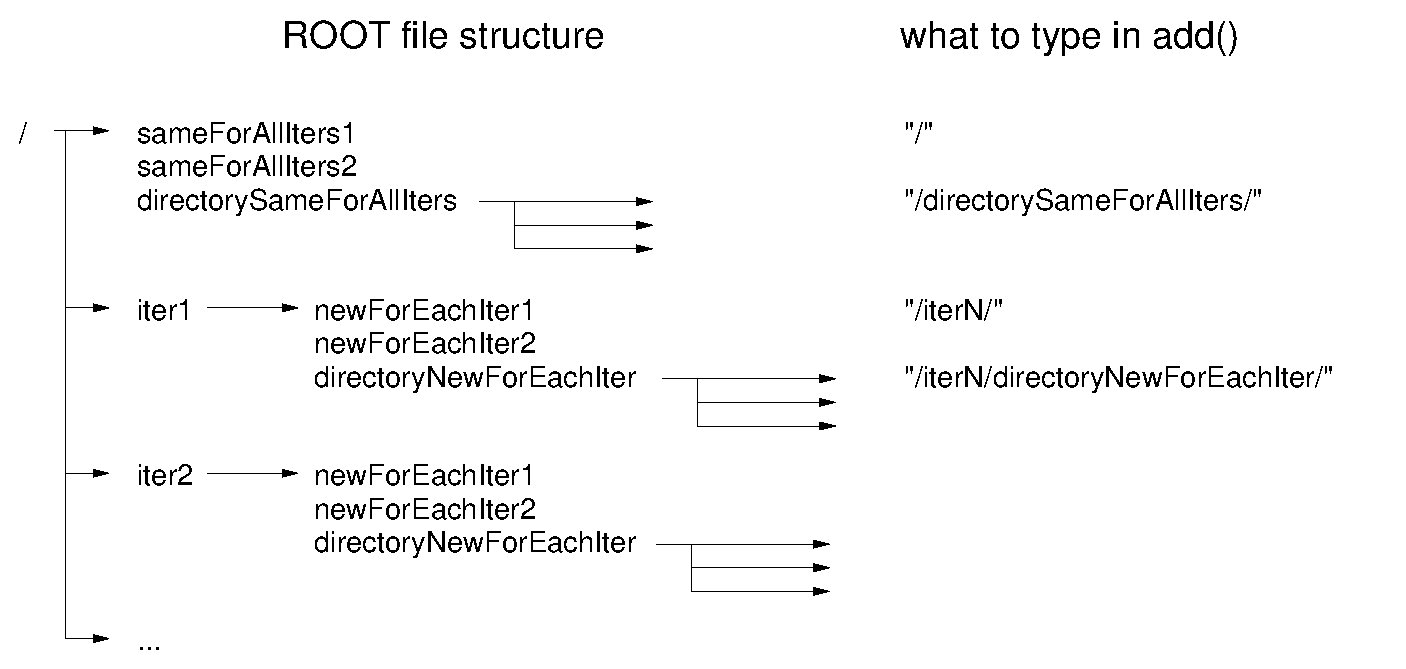
\includegraphics[width=\linewidth]{rootfile}

\vfill
Nothing more is needed for collection jobs
\end{frame}

\begin{frame}
\frametitle{Status}
What works (tested with hundreds of events):
\begin{itemize}
  \item Loading an arbirtary number of modules
  \item Arbitrarily-deep ROOT directory structure
  \item Iteration (via {\tt AlignmentProducer.maxLoops} and/or multiple cmsRun invocations)
  \item Merging histograms/profiles from a distributed job
  \item Generating histograms from selected Alignables
\end{itemize}

\vfill
What's next:
\begin{itemize}
  \item Add lots of plots to a new module
  \item Use it for CSC internal alignment with MTCC data
\end{itemize}
\end{frame}

\section*{}
\begin{frame}
\Huge
\begin{center}--- New Topic ---\end{center}
\end{frame}

\section*{Database Geometry Monitoring --- Dmitry Yakorev}

\begin{frame}
\frametitle{Monitoring differences in geometry between alignments}
\begin{columns}
\column{0.03\linewidth}
vs.\ $R$ \\

\vspace{1 cm}
vs.\ $\phi$ \\

\vspace{1 cm}
vs.\ $Z$ \\
\column{0.98\linewidth}
\includegraphics[width=\linewidth]{screen_shot.png}
\end{columns}

\vfill
\hfill $(\vec{x_1}-\vec{x_2})$ \hfill $(\vec{x_1}-\vec{x_2})\cdot\hat{\phi}$ \hfill $(\vec{x_1}-\vec{x_2})\cdot\hat{Z}$ \hfill
\end{frame}

\begin{frame}
\frametitle{Status}

Basic structure:
\begin{itemize}
  \item Compiled C++ ROOT GUI
  \item Forks {\tt cmsRun} processes which read SQLite files/the database
\end{itemize}

What works:
\begin{itemize}
  \item Loading two geometry files
  \item Calculating and displaying translation differences
  \item Tabs to switch between plots
\end{itemize}

\vfill
What's next:
\begin{itemize}
  \item Read from multiple databases--- plot versus time
  \item Represent differences in rotation angles
  \item A different framework?  DQM?  Iguana?  Compile database access into ROOT GUI?
\end{itemize}
\end{frame}

\section*{}
\begin{frame}
\Huge
\begin{center}--- New Topic ---\end{center}
\end{frame}

\section*{Alignable tree for muon system --- Jim Pivarski}

\begin{frame}
\frametitle{AlignableDets and AlignableDetUnits in the Muon System}
\begin{center}
\includegraphics[width=0.85\linewidth]{aligabletree}
\end{center}
\begin{itemize}
\item Without Gero's fix, we calculate DT corrections on layer plane, then apply to superlayer plane
\end{itemize}
\end{frame}

\section*{}
\begin{frame}
\Huge
\begin{center}--- New Topic ---\end{center}
\end{frame}

\section*{1D DT Hits --- Jim Pivarski}

\begin{frame}
\frametitle{1D treatment of DT hits}
\begin{center}
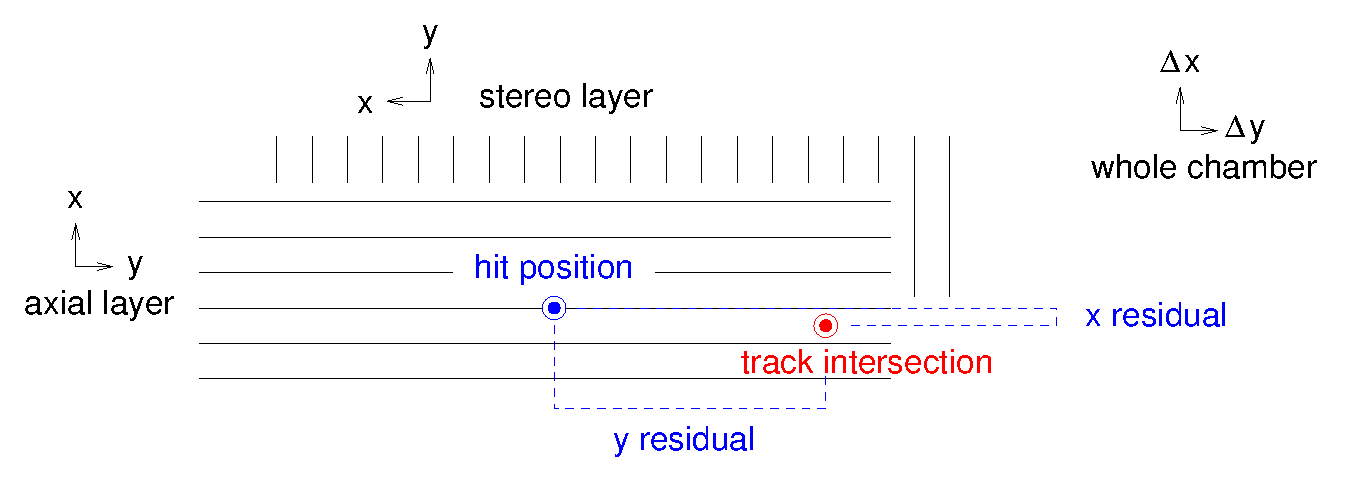
\includegraphics[width=0.9\linewidth]{axialstereo}
\end{center}

\vspace{-0.5 cm}
\begin{itemize}
\item Local $x$, $y$ residuals are correctly transformed into $\Delta x$, $\Delta y$ alignment corrections
\item Axial $y$ and stereo $y$ contain no alignment info
\item ParameterSelector can turn off $\Delta y$ corrections, not $y$ residuals
\item In HIP, I want to add: {\tt if(DT) \{residInverse.yy = 0;\}}
\item How should we express ``{\tt if(DT)}''?
\end{itemize}
\end{frame}

\begin{frame}
\frametitle{This has significant consequences!}

Without {\tt residInverse.yy = 0}, DT corrections are \textcolor{red}{\fbox{${\mathcal O}(\mbox{1 m})$!}}

\vfill
With {\tt residInverse.yy = 0}, they are as expected:

\vfill
\begin{columns}
\column{0.35\linewidth}
\includegraphics[width=\linewidth]{init_alignments_x}

\column{0.35\linewidth}
\includegraphics[width=\linewidth]{x_alignments_x}

\column{0.35\linewidth}
\includegraphics[width=\linewidth]{phiz_alignments_phiz}
\end{columns}
\end{frame}

\section*{}

\begin{frame}
\frametitle{Summary}
\begin{itemize}\setlength{\itemsep}{0.75 cm}
\item Monitor plugins are in CVS:

Alignment/CommonAlignmentMonitor V00-00-00 \\
Alignment/CommonAlignmentProducer V00-15-00

\item Work has begun on a database monitoring tool

\item Muon DTs are a use case for Gero's AlignableDet / AlignableDetUnit fix

\item We also need to ignore alignment corrections coming from DT $y$ residuals

\end{itemize}
\label{numpages}
\end{frame}

\end{document}
